\section{Architectural Design} \label{sec:arch-design}

In this section, we will show the proposed architecture for our system, that allow us to give a more complete and general idea of the entire system and a better view of the relation with external components.

\subsection{Overview} \label{subsec:overview}
Now we are going to present an overall description of the architecture of our system. We propose a 4-tier architecture, following the model of the \acl{jee} architecture, shown in Figure \ref{fig:jeearch}. The \textbf{client}, usually a web client or an application client, runs on the client machine. Instead the \textbf{business} code, which is logic that solves or meets the needs of a particular business domain (such as banking) runs on the server machine, as it happens for the \textbf{Web-tier}. The \textbf{\acl{eis}-tier} includes enterprise infrastructure systems, such as the database and legacy systems, and it runs on a third dedicated machine. \\For sake of simplicity, in this document the web client and the mobile application are treated as one entity. For this reason, each communication between server and client will pass through the Web-tier.
\\ \acs{jsf} technology is a server-side component framework for building Java technology-based web applications and we will use it for the dynamic web pages.
As far as the communication with the mobile application is concerned, we will consider an implementation of the \acs{rest} paradigm.\\
\newline
In the following part, we will give a more accurate and detailed description of this 4-tier architecture.

\begin{itemize}

\item[--]\textbf{Client-tier}: This tier component are the Application Clients and Web Browsers. They both typically have a \acs{gui}, since they interact with the actors.

\item[--]\textbf{Web-tier}: This tier component has the task to manage the requests sent by the Client-tier and to forward these requests to the Business-tier. In a similar way, the Web-tier elaborates the contents generated by the Business-tier and it sends these contents to the Client-tier in a way that this tier components can render the information received.

\item[--]\textbf{Business-tier}: This tier represents the core of the whole system. This tier components contain the logic that solves or meets the needs of a particular business domain such as banking, retail, or finance, is handled by Enterprise Java Beans. They receive data from client programs, processes it, and sends it to the \acs{eis}-tier for storage. An Enterprise Java Bean also retrieves data from storage, processes it, and sends it back to the client program.
All the application logic resides here under the form of Enterprise Java Beans and Java Entities. This tier is connected to the Database through a Java Persistence API.

\item[--]\textbf{\acs{eis}-tier}: This tier components are usually database and legacy systems, where the entire system stores the needed persistent information.

\end{itemize}

\begin{figure}[htbp]
\centering
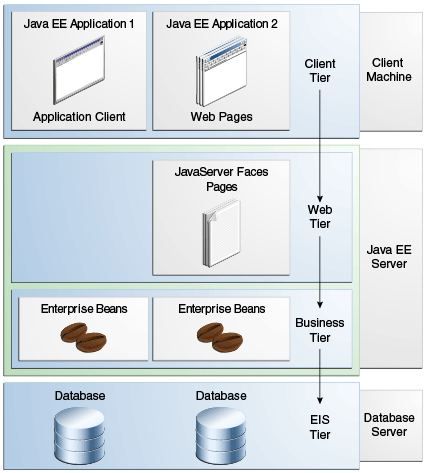
\includegraphics[width=0.8\textwidth]{Images/jeett_dt_001.png}
\caption{JEE 4-tier architecture}
\label{fig:jeearch}
\end{figure}
\clearpage

\subsection{Interactions with External Components} \label{subsec:comp-extern}
The diagram in Figure \ref{fig:connection} shows the interactions between our system and all the external components, that are the \textbf{Mapping Service}, the \textbf{Bank} and the \textbf{Car System}.

\begin{figure}[htbp]
\centering
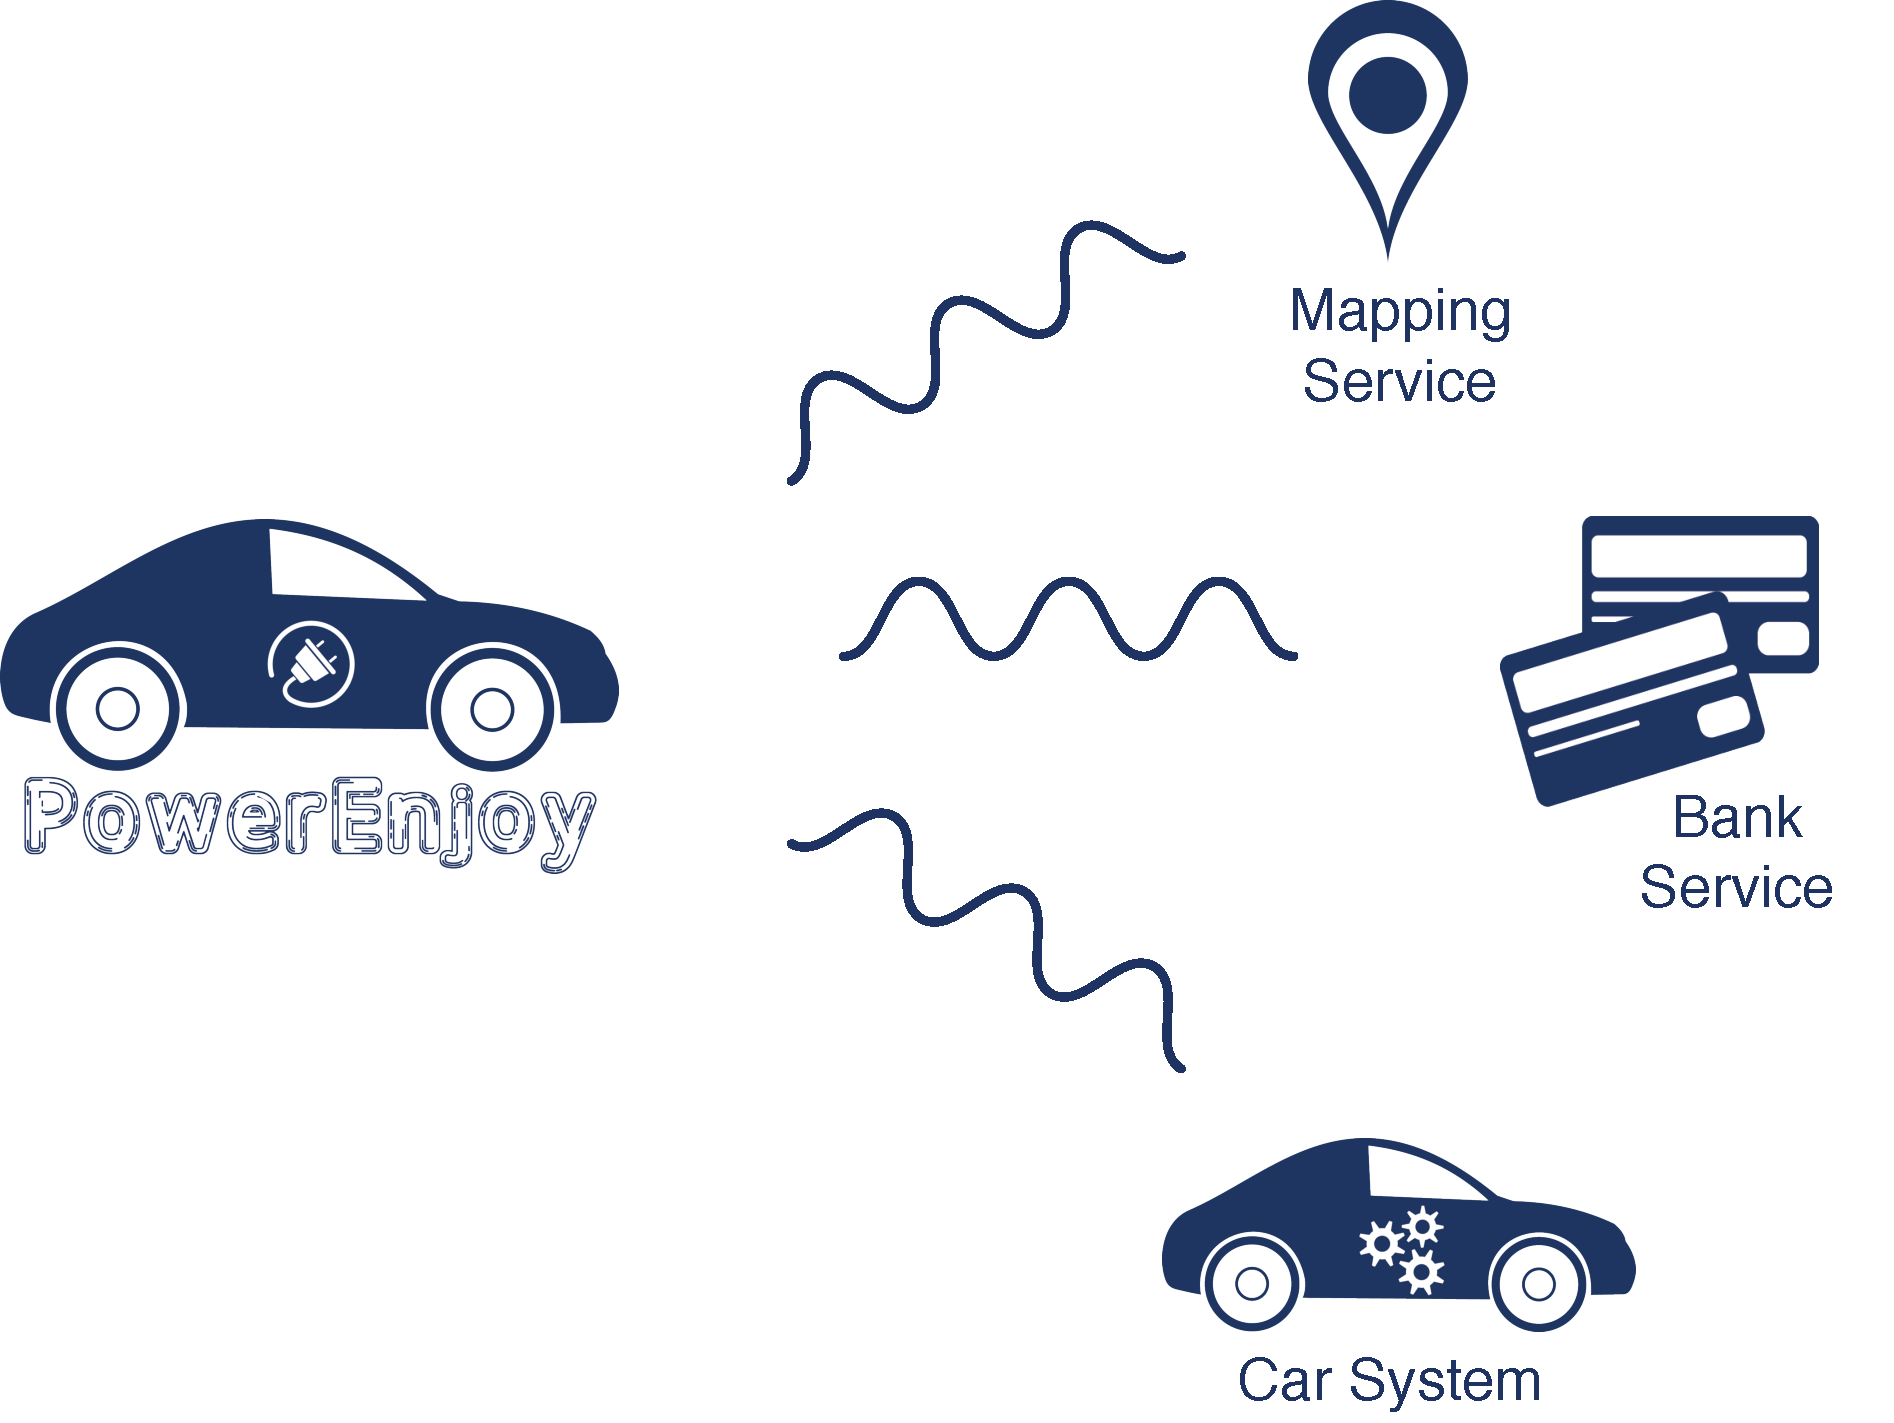
\includegraphics[width=0.8\textwidth]{Images/Connection}
\caption{Interactions between our system and the external components}
\label{fig:connection}
\end{figure}
\clearpage

\clearpage

\subsection{Internal High Level Components and their Interaction} \label{subsec:comp-inter}

The diagram in Figure \ref{fig:high-comp} shows the conceptual high level architecture we propose for our system.
\vspace{18pt}
\begin{figure}[htbp]
\centering
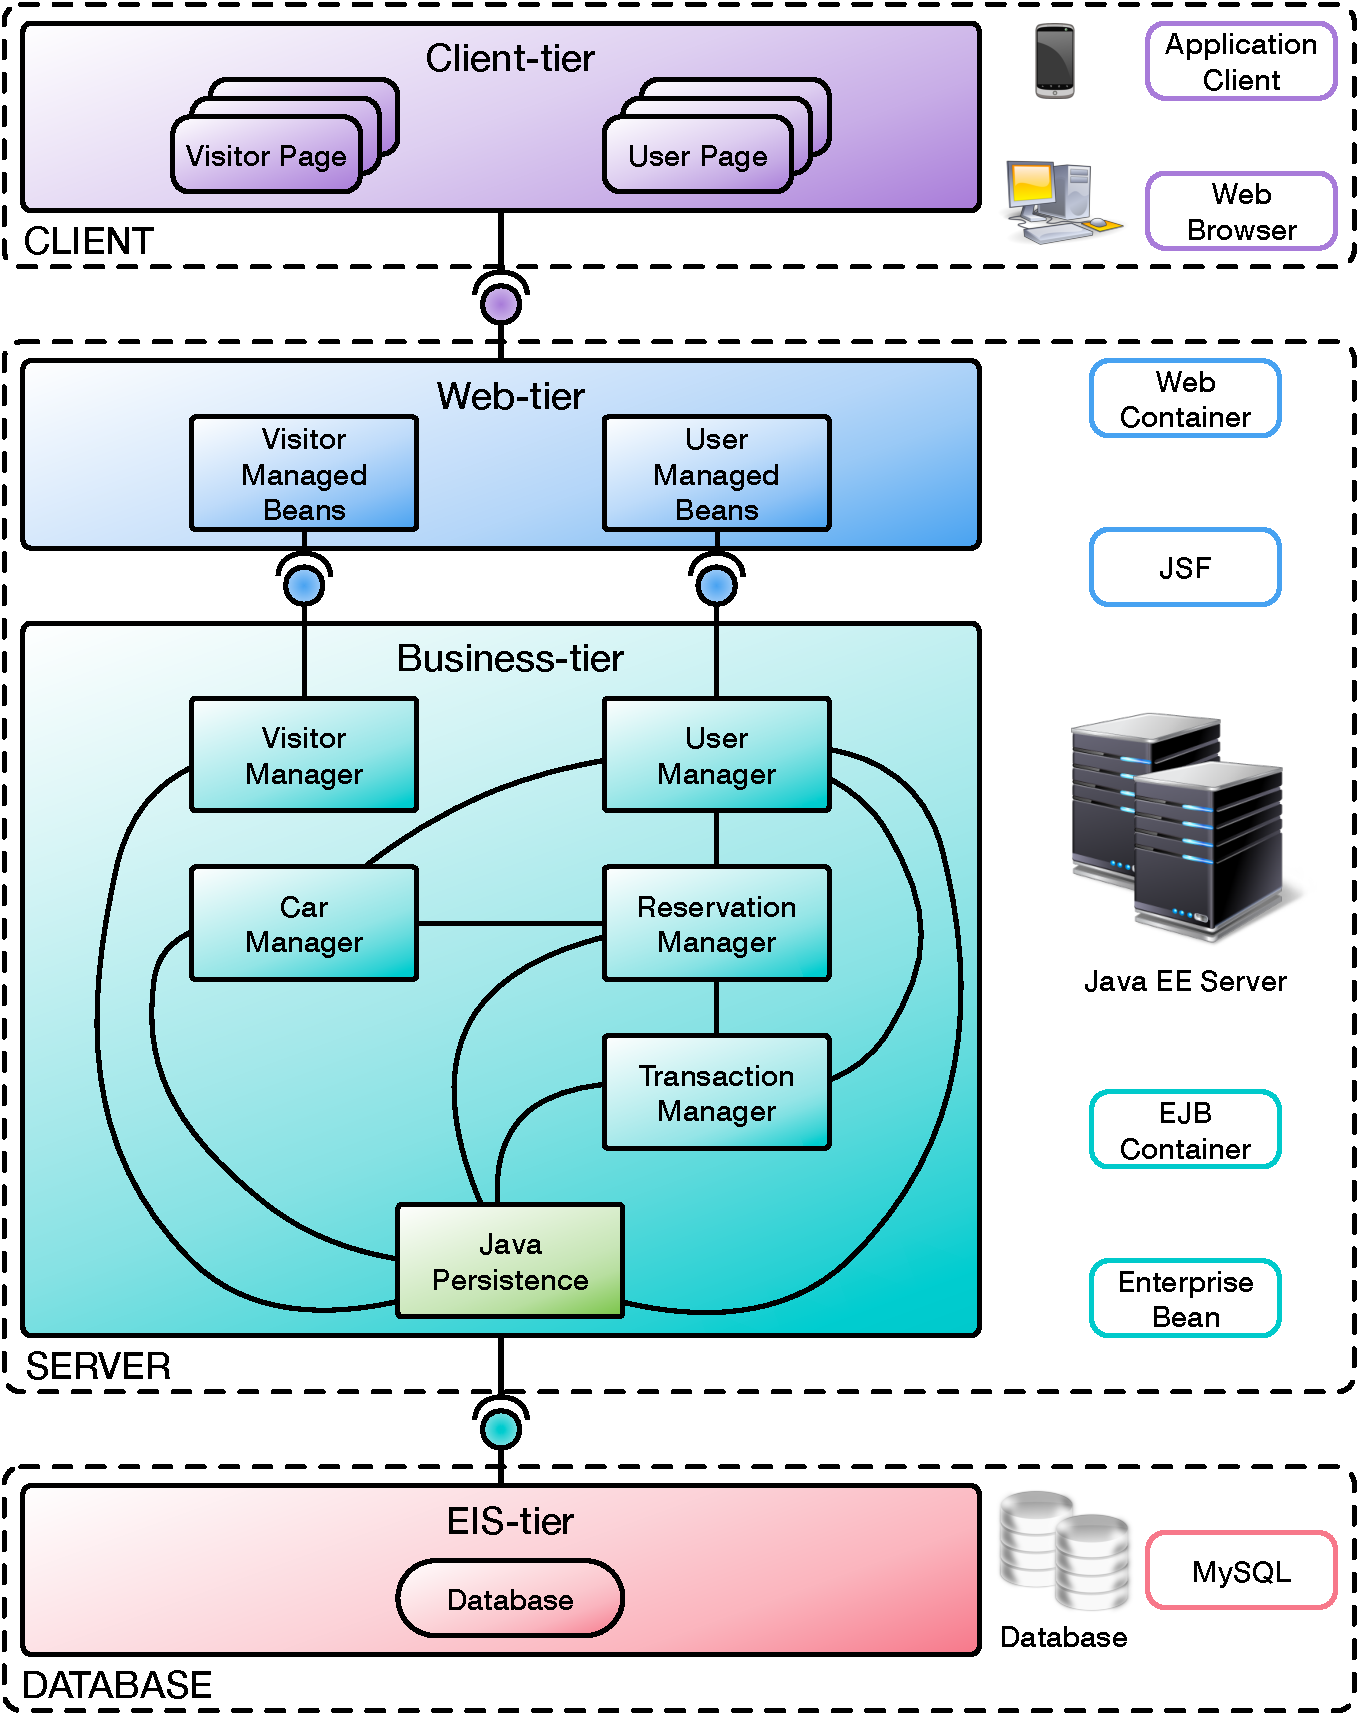
\includegraphics[width=0.85\textwidth]{Images/HighLevelComponents.pdf}
\vspace{10pt}
\caption{High Level Components and their Interaction of PowerEnjoy}
\label{fig:high-comp}
\end{figure}
\clearpage

\subsection{Component view} \label{subsec:comp-view}
In this subsection, we are going to analyze more in details the component we have just introduced.

\myparagraph{Client component} 
\newline
The first component we are going to analyze is shown in Figure \ref{fig:client}: the Client component provides a way for users to handle tasks that require a richer user interface than can be provided by a markup language (HTML, XML, and so on).
The clients usually do not query databases, execute complex business rules, or connect to legacy applications: such operations are off-loaded to enterprise beans executing on the server, where they can leverage the security, speed, services, and reliability of Java EE server-side technologies.
The Client component present different interfaces: each of them display the user only the pages for which he has permissions. 
Each interface is a subcomponent of the Client component.

\vspace{52pt}
\begin{figure}[htbp]
\centering
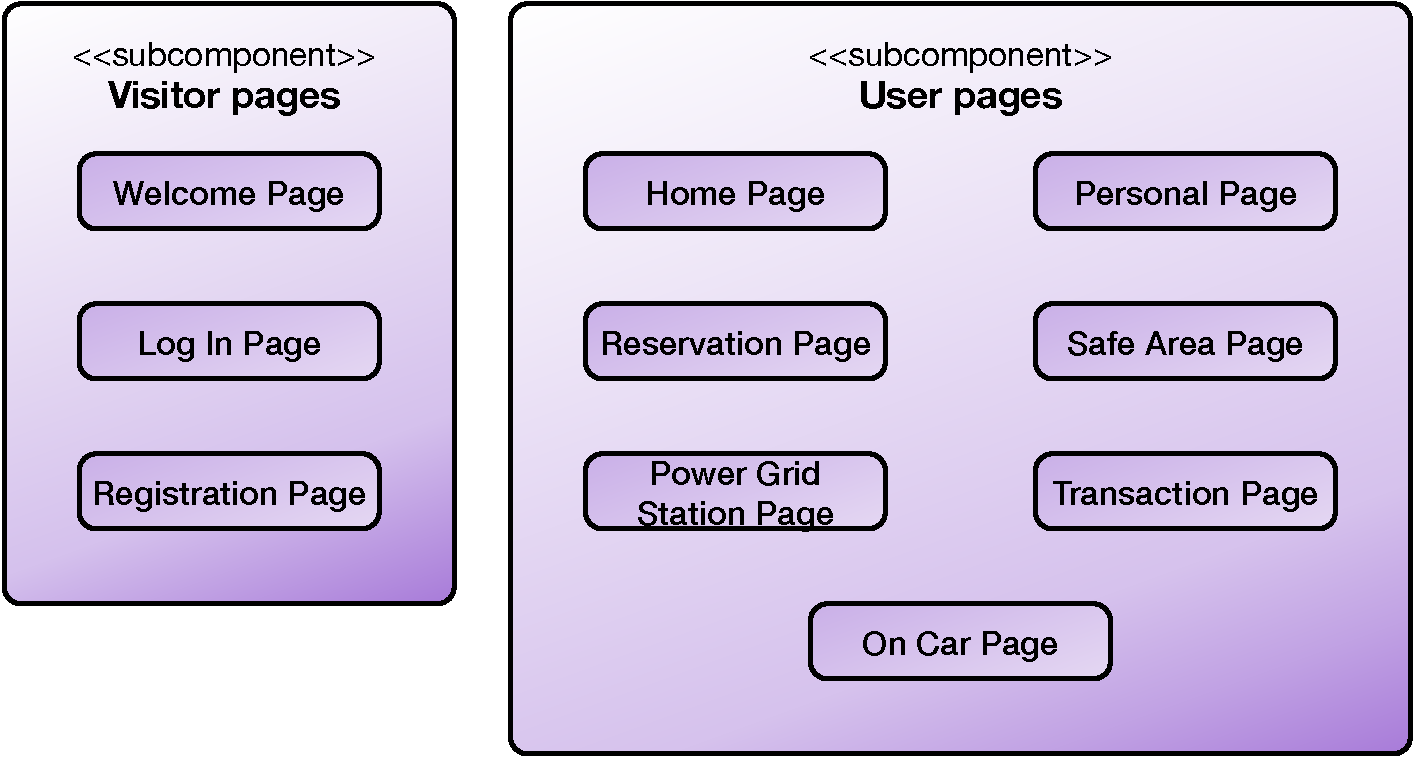
\includegraphics[width=0.85\textwidth]{Images/ClientComponent.pdf}
\vspace{10pt}
\caption{Client component and its subcomponents}
\label{fig:client}
\end{figure}
\clearpage

\myparagraph{Web component} 
\newline
The second component we are going to analyze is shown in Figure \ref{fig:web}: the Web component generates dynamic web pages containing XHTML. Moreover, it implements \acl{jsf} technology, a common user interface component framework for web applications.
The Web component includes also JavaBeans components, one for each group of pages, in order to manage the user input and then send that input to enterprise beans running in the Business-tier for processing.

\vspace{104pt}
\begin{figure}[htbp]
\centering
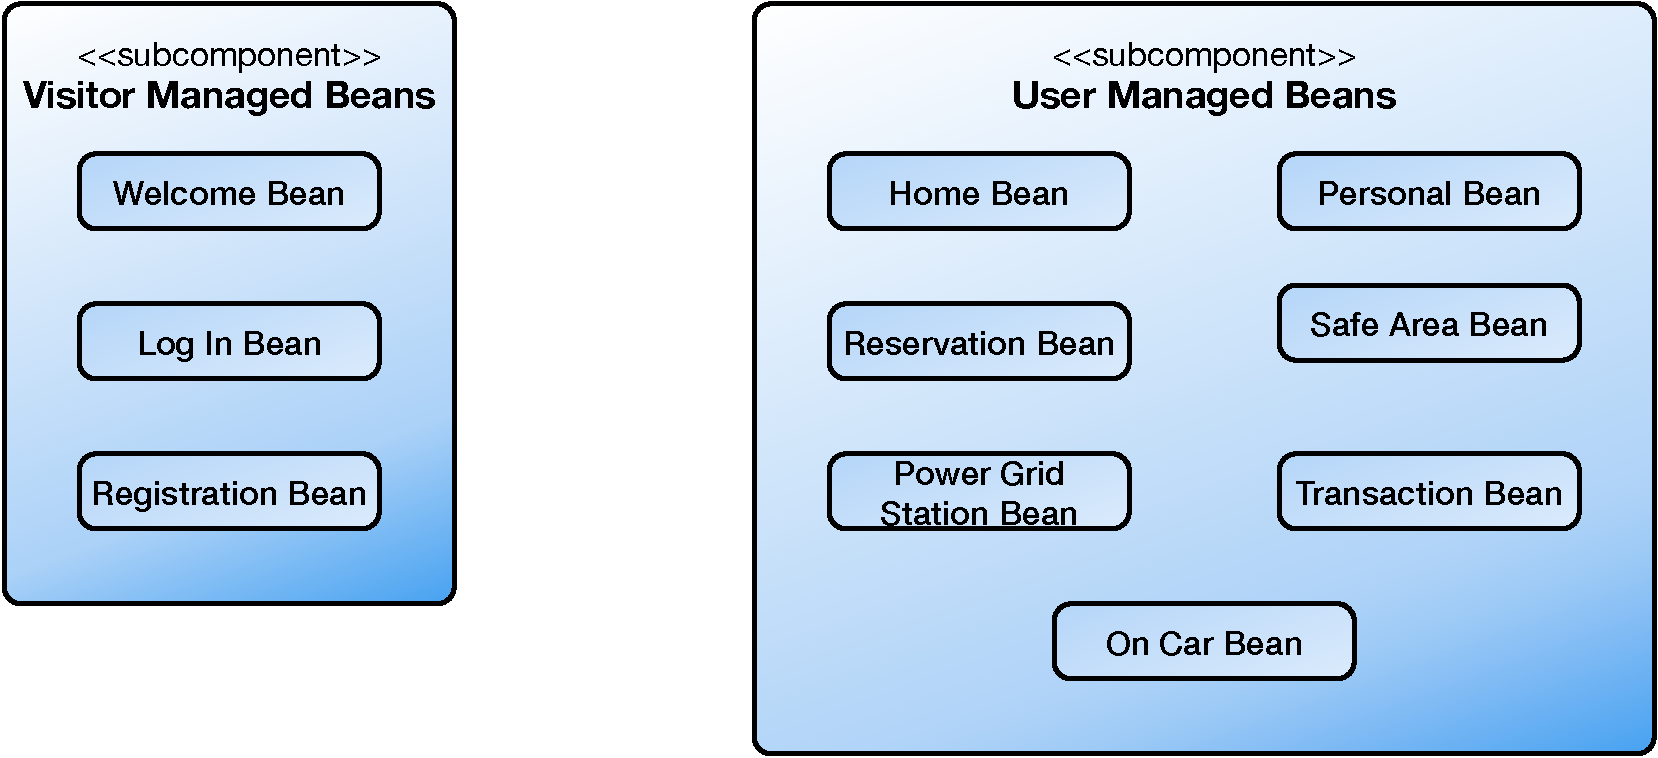
\includegraphics[width=0.85\textwidth]{Images/WebComponent.pdf}
\vspace{10pt}
\caption{Web component and its subcomponents}
\label{fig:web}
\end{figure}
\clearpage

\myparagraph{Business Logic component} 
\newline
The third component we are going to analyze is shown in Figure \ref{fig:business}: the Business component. It includes \acl{ejb}s that are a server-side component encapsulating the business logic of an application. An \acs{ejb} is a body of code that has fields and methods to implement modules of business logic. You can think of it as a building block that can be used to execute business logic on the Java EE server.
The \textbf{business logic} is the code that fulfills the purpose of the application.

Another task performed by the Business Logic Component is to transfer and processes data between the Client component and the Java Persistence Entity, which holds the information of the system data model and it has to store and retrieve information from the database.

In this document, we focus only on the fundamental elements needed in order to manage the basic functionalities. However, further details and functionality will be added during the development. Here we show the reader some of them.

\begin{itemize}
\item The \textbf{Visitor Manager} has to perform the following functionalities:
	\begin{itemize}
	\item check the validity and correctness of user's information;
	\item create a new user and save them into the database;
	\item check if the Log In is valid; if so, it has to authenticate the user.
	\end{itemize}
\item The \textbf{User Manager} has to manage the user's profile and the geolocalization services.
\item The \textbf{Car Manager} has to manage the car status and position.
\item The \textbf{Reservation Manager} has to allow a user to reserve a free car and it has to keep track of all the related information, for example duration and number of passengers.
\item The \textbf{Transaction Manager} has to charge the user for its reservation and apply eventual discount or penalties.
\end{itemize}
\clearpage

\begin{figure}[htbp]
\centering
\vspace{104pt}
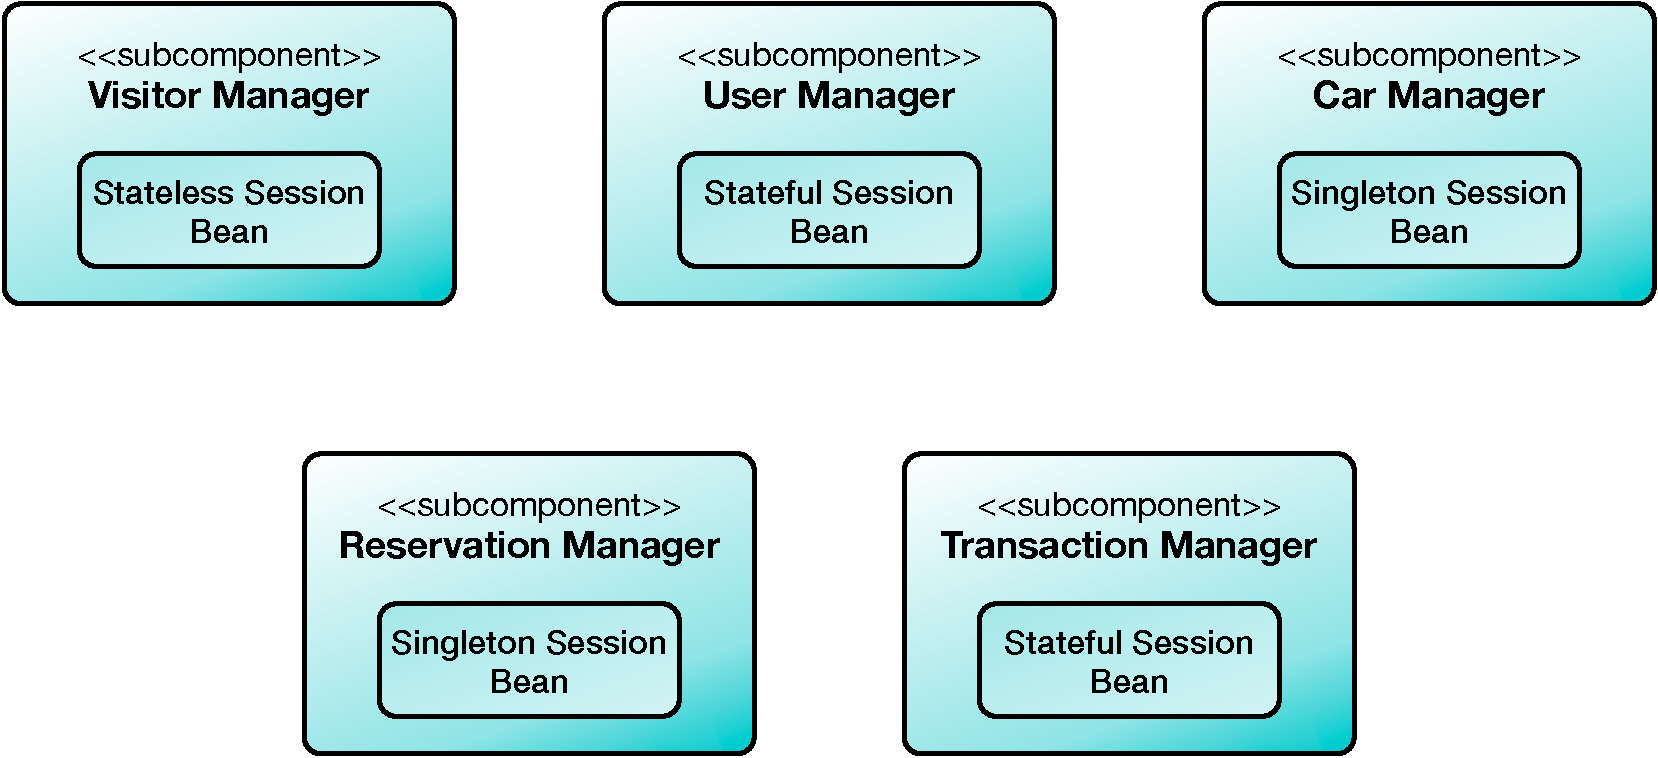
\includegraphics[width=0.85\textwidth]{Images/BusinessLogicComponent.pdf}
\vspace{10pt}
\caption{Business Logic component and its subcomponents}
\label{fig:business}
\end{figure}
\clearpage

\myparagraph{Database component} 
\newline
The last component we are going to analyze is shown in Figure \ref{fig:database}: the Database component. In order to show the conceptual architecture of this component, we used an \acl{er} model, useful to highlight the entities of the system and to specify the relationships that can exist between instances of those entity types.

\begin{figure}[htbp]
\centering
\vspace{24pt}
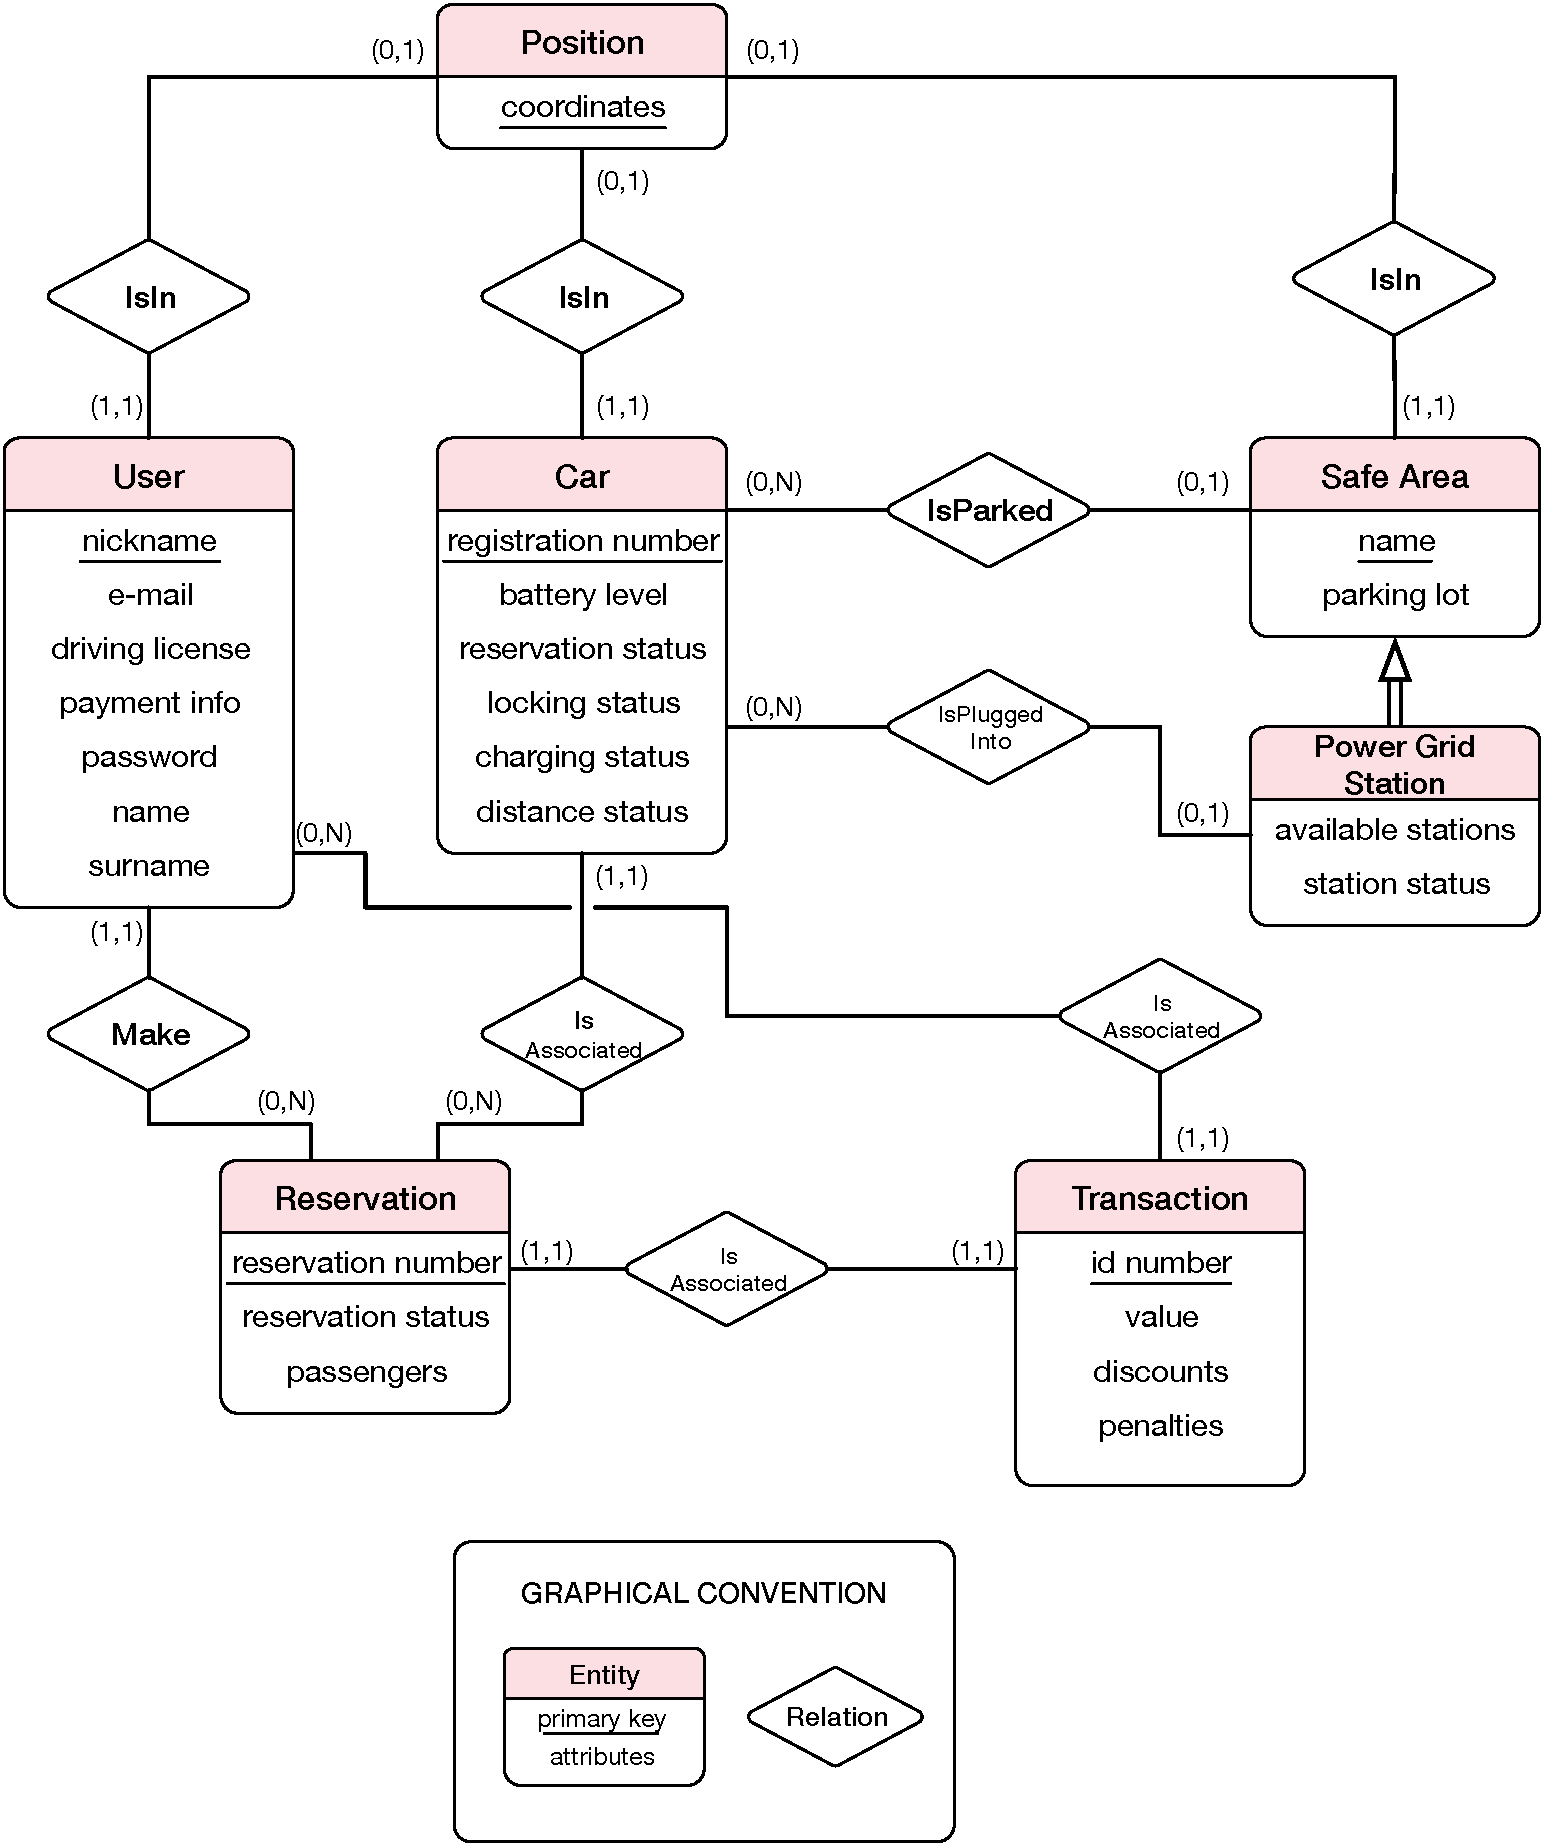
\includegraphics[width=0.85\textwidth]{Images/DatabaseComponent.pdf}
\vspace{10pt}
\caption{\acs{er} model of the Database component}
\label{fig:database}
\end{figure}
\clearpage

\subsection{Deployment view} \label{subsec:depl-view}

The diagram in Figure \ref{fig:deployment} shows the deployment view of the software product. In this early stage, we choose to keep our diagram simple and to only highlight a first distinction between the client machine, the server machine and the database machine.
In the next steps of the development, we will detail in a more in specific way the hardware architecture, identifying the hardware components on which the software layer will be deployed.

\begin{figure}[htbp]
\centering
\vspace{12pt}
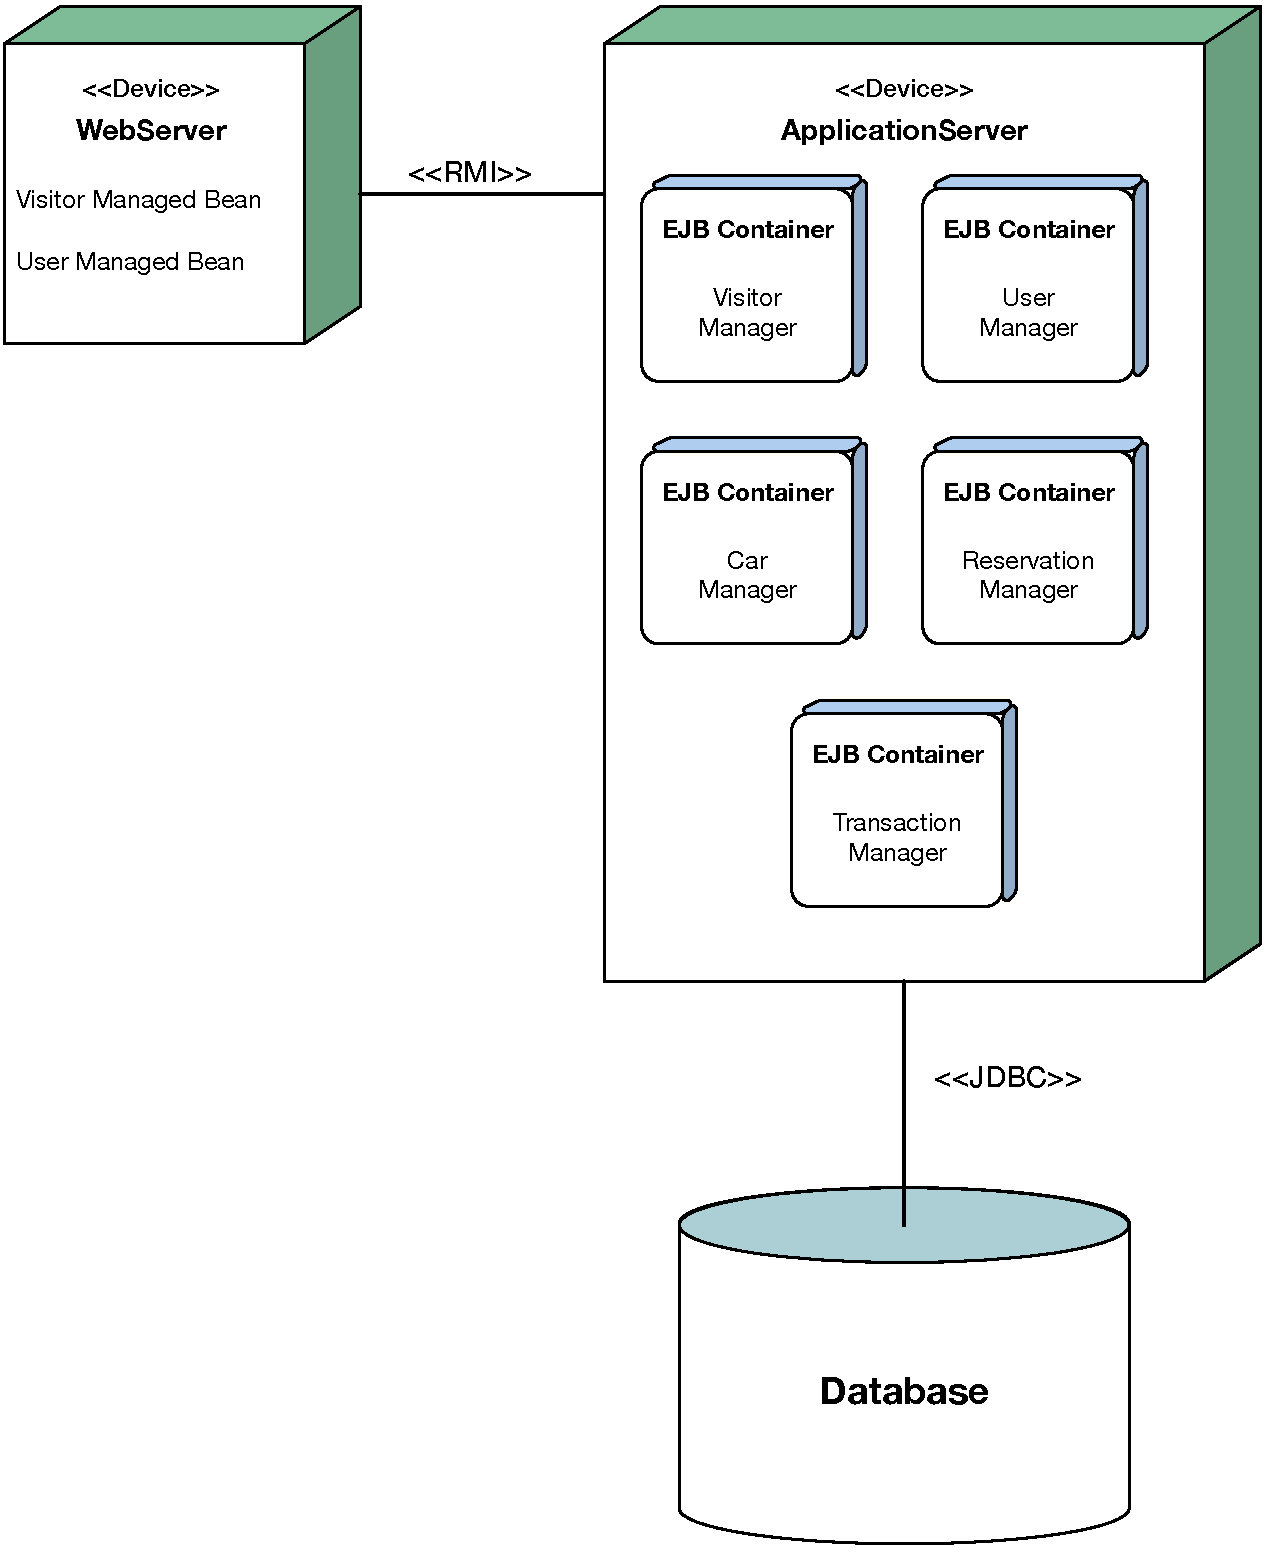
\includegraphics[width=0.85\textwidth]{Images/Deployment.pdf}
\vspace{10pt}
\caption{Diagram showing the Deployment view}
\label{fig:deployment}
\end{figure}
\clearpage

\subsection{Runtime view} \label{run-view}
%You can use sequence diagrams to describe the way components interact to accomplish specific tasks typically related to your use cases

In the following subsection, we will show the reader some diagrams that  represent the runtime view of PowerEnjoy system: they describe in a simple way the interaction and the behaviour of the component previously described in order to make possible the main functionalities of our system.

\myparagraph{Log In and Registration runtime view}
\newline
The diagram represented in Figure \ref{fig:login} shows the components involved in the login and registration activities and their interactions.

\begin{figure}[htbp]
\centering
\vspace{52pt}
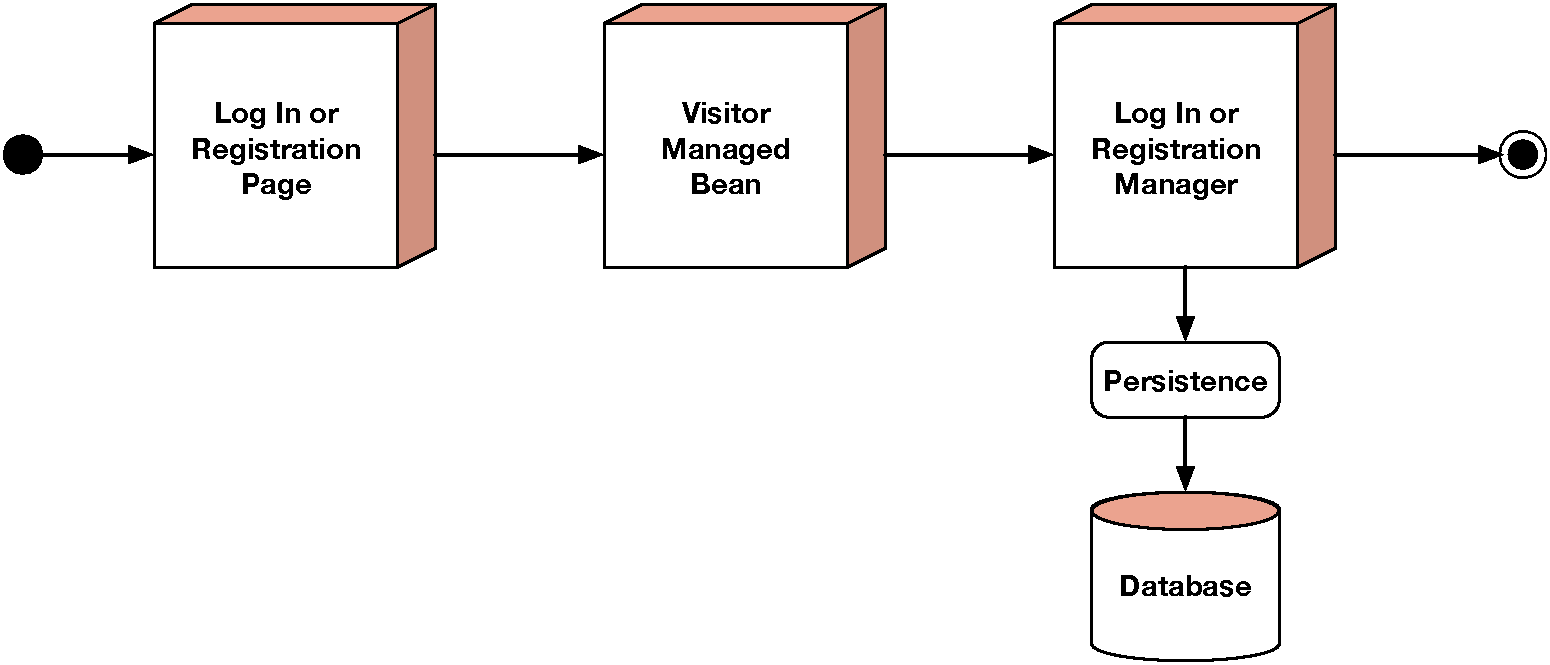
\includegraphics[width=0.85\textwidth]{Images/LogInRun.pdf}
\vspace{10pt}
\caption{Diagram showing the Log In and Registration runtime view}
\label{fig:login}
\end{figure}
\clearpage

\myparagraph{Modification of User's account runtime view}
\newline
The diagram represented in Figure \ref{fig:modify} shows the components involved in the modification of user's account and their interactions.

\begin{figure}[htbp]
\centering
\vspace{104pt}
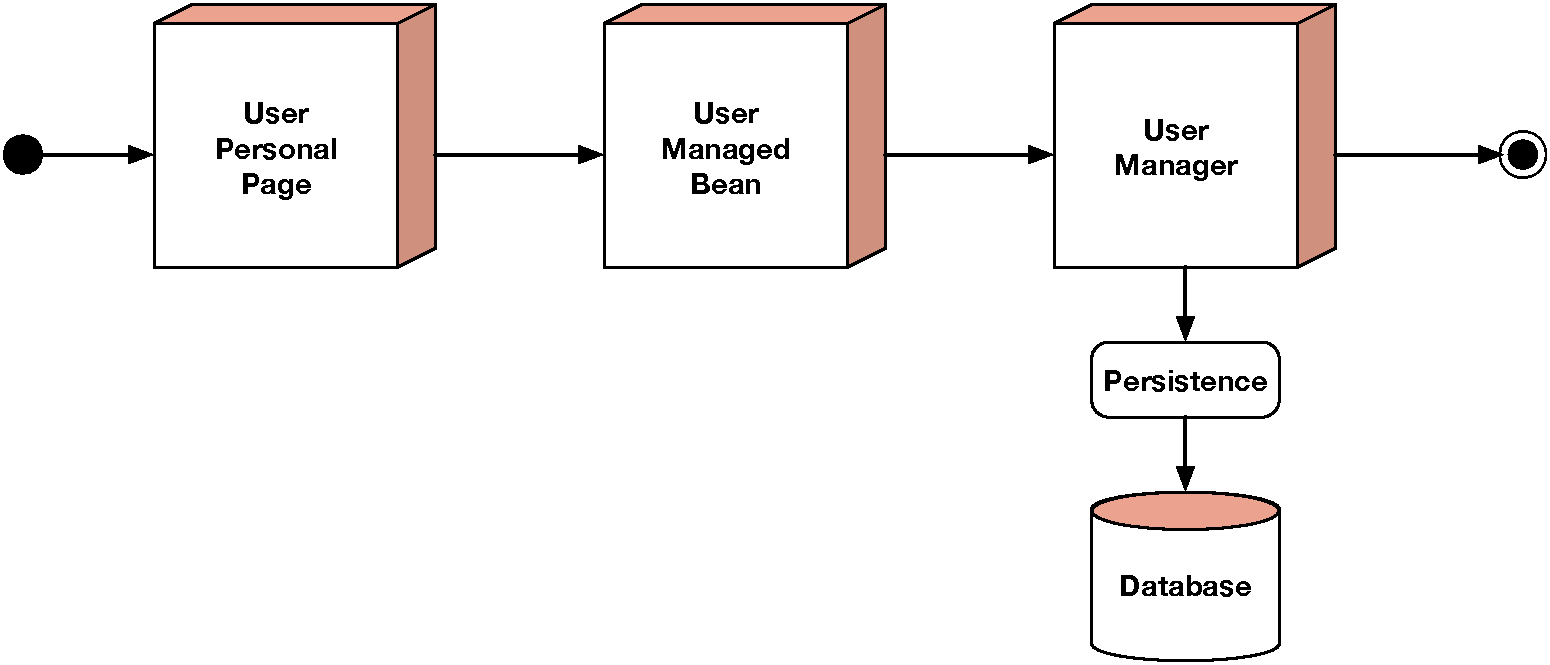
\includegraphics[width=0.85\textwidth]{Images/ModifyRun.pdf}
\vspace{10pt}
\caption{Diagram showing the Modification of User's account runtime view}
\label{fig:modify}
\end{figure}
\clearpage

\myparagraph{Car Reservation runtime view}
\newline
The diagram represented in Figure \ref{fig:reserve} shows the components involved in the car reservation and their interactions.

\begin{figure}[htbp]
\centering
\vspace{104pt}
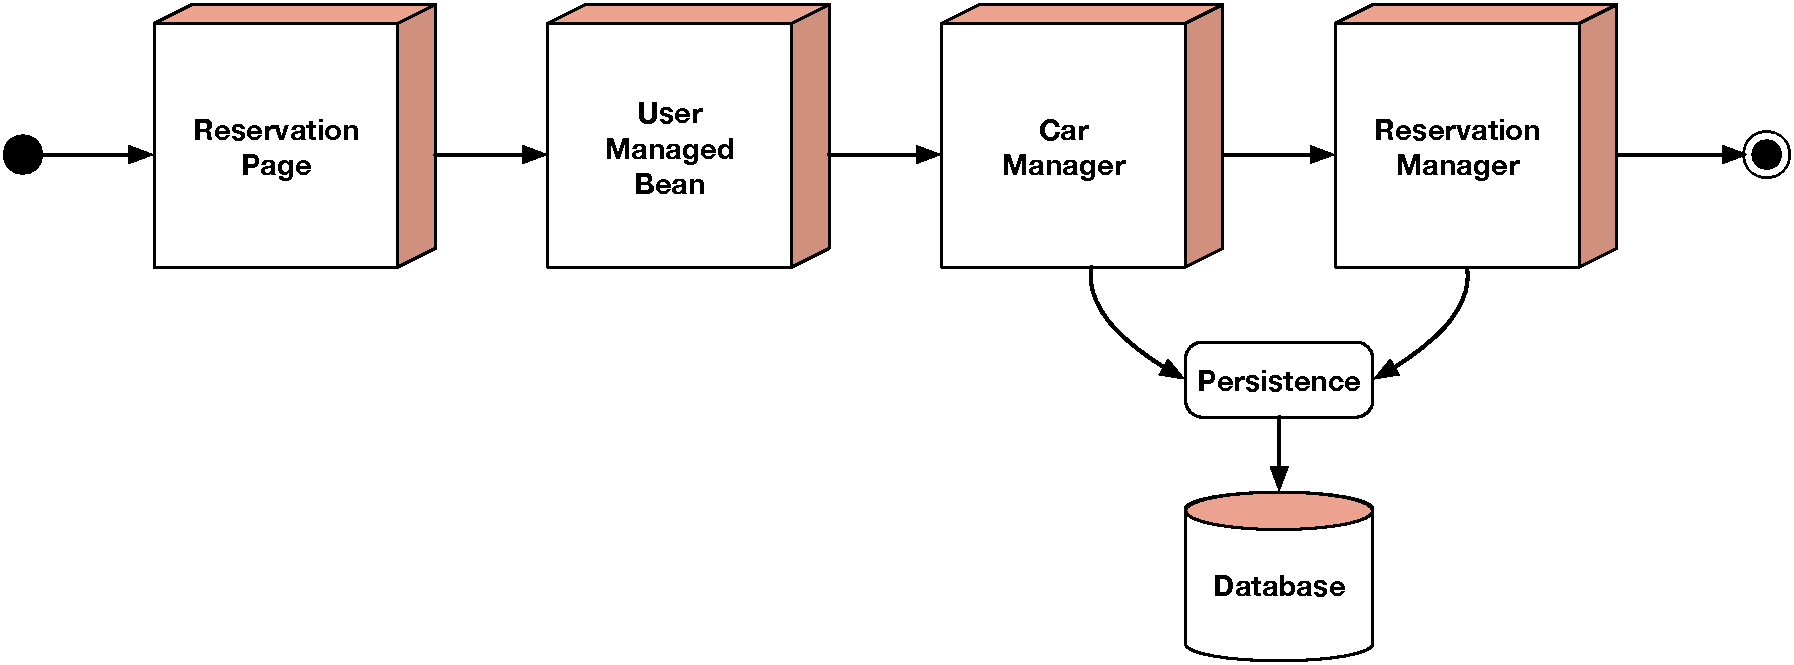
\includegraphics[width=0.85\textwidth]{Images/ReserveRun.pdf}
\vspace{10pt}
\caption{Diagram showing the Car Reservation runtime view}
\label{fig:reserve}
\end{figure}
\clearpage

\myparagraph{Safe Area and Power Grid Station display runtime view}
\newline
The diagram represented in Figure \ref{fig:display} shows the components involved in the display of safe areas and power grid stations and their interactions.

\begin{figure}[htbp]
\centering
\vspace{104pt}
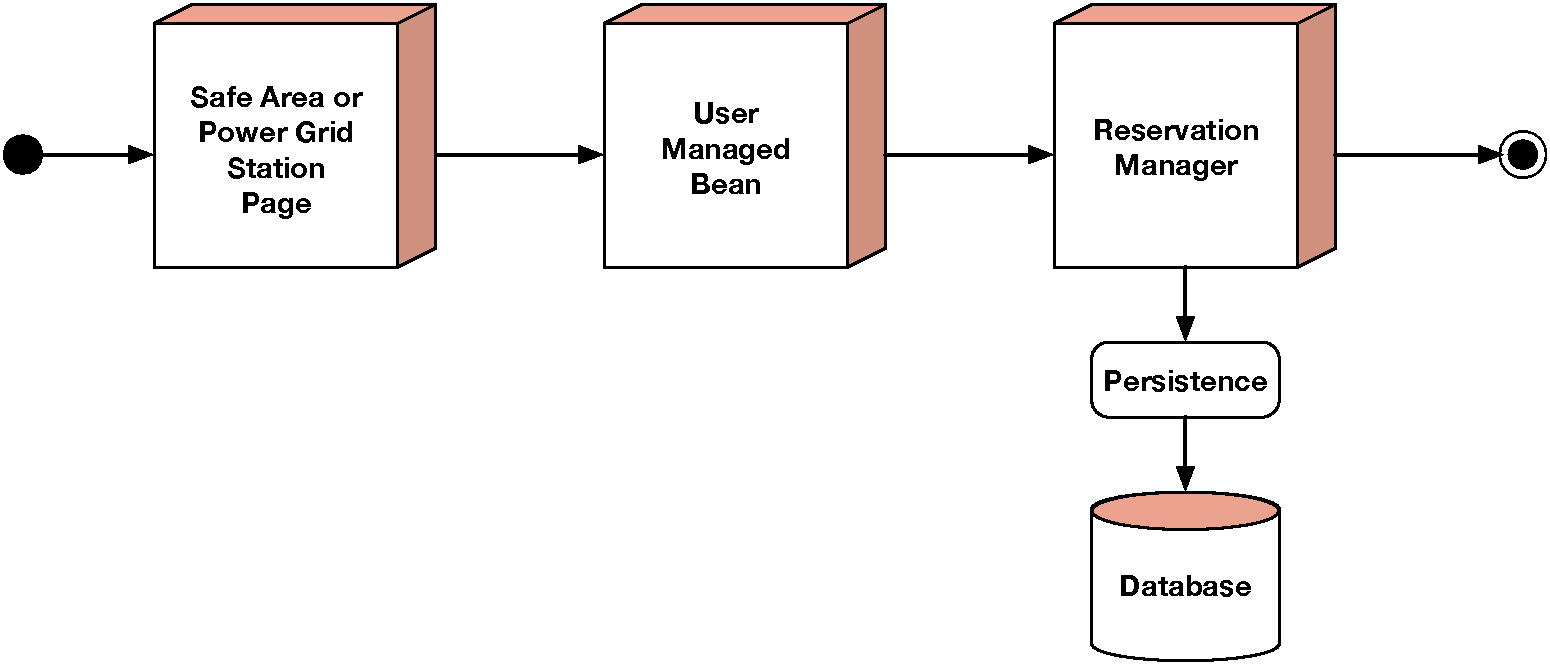
\includegraphics[width=0.85\textwidth]{Images/DisplayRun.pdf}
\vspace{10pt}
\caption{Diagram showing the Safe Area and Power Grid Station display runtime view}
\label{fig:display}
\end{figure}
\clearpage

\myparagraph{Details during the Ride display runtime view}
\newline
The diagram represented in Figure \ref{fig:ride} shows the components involved in the display of the details during the ride and their interactions.

\begin{figure}[htbp]
\centering
\vspace{104pt}
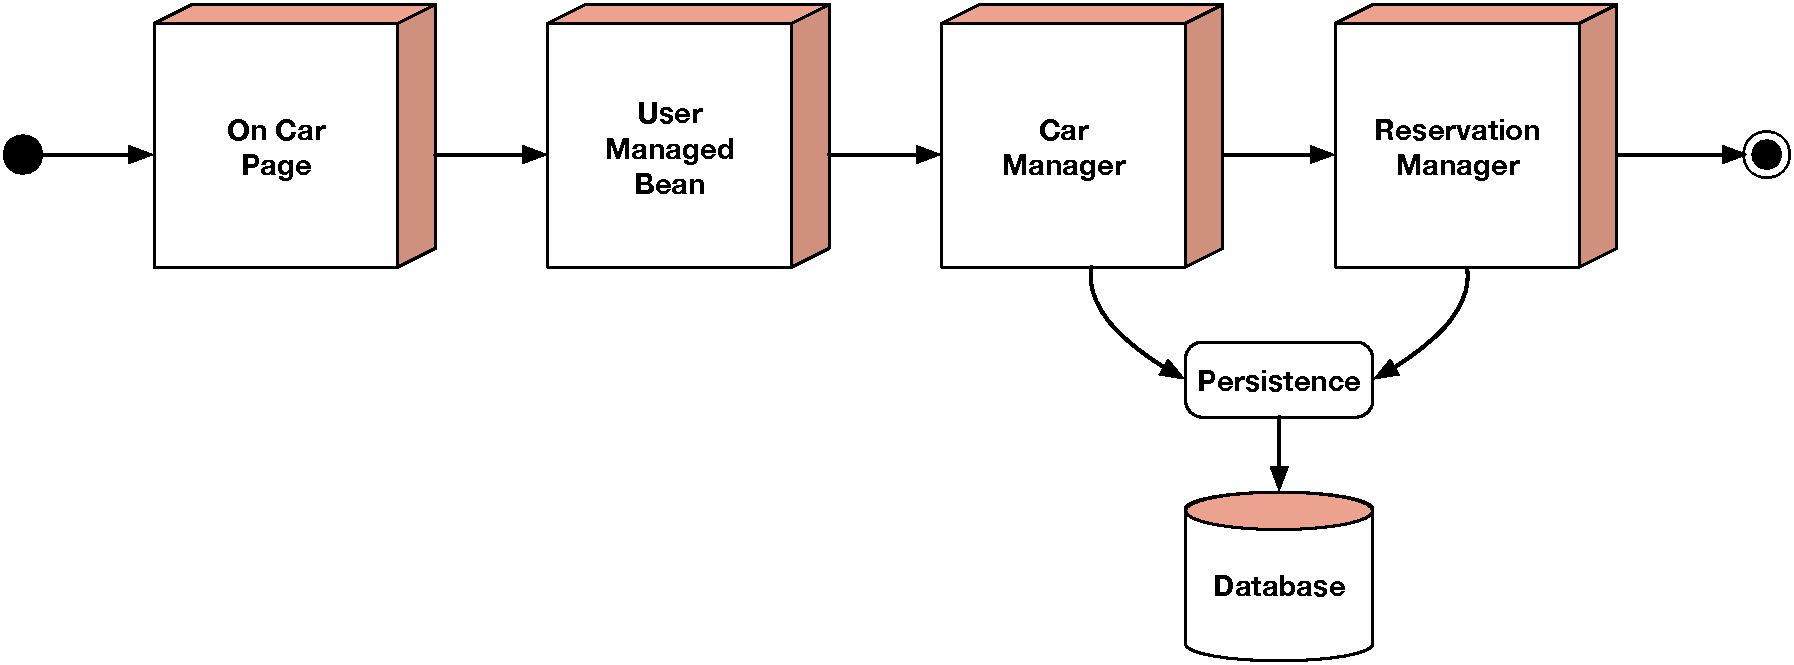
\includegraphics[width=0.85\textwidth]{Images/RideRun.pdf}
\vspace{10pt}
\caption{Diagram showing the Details during the Ride display runtime view}
\label{fig:ride}
\end{figure}
\clearpage

\myparagraph{Fee computation and display runtime view}
\newline
The diagram represented in Figure \ref{fig:fee} shows the components involved in the computation and display of the fee and their interactions.

\begin{figure}[htbp]
\centering
\vspace{104pt}
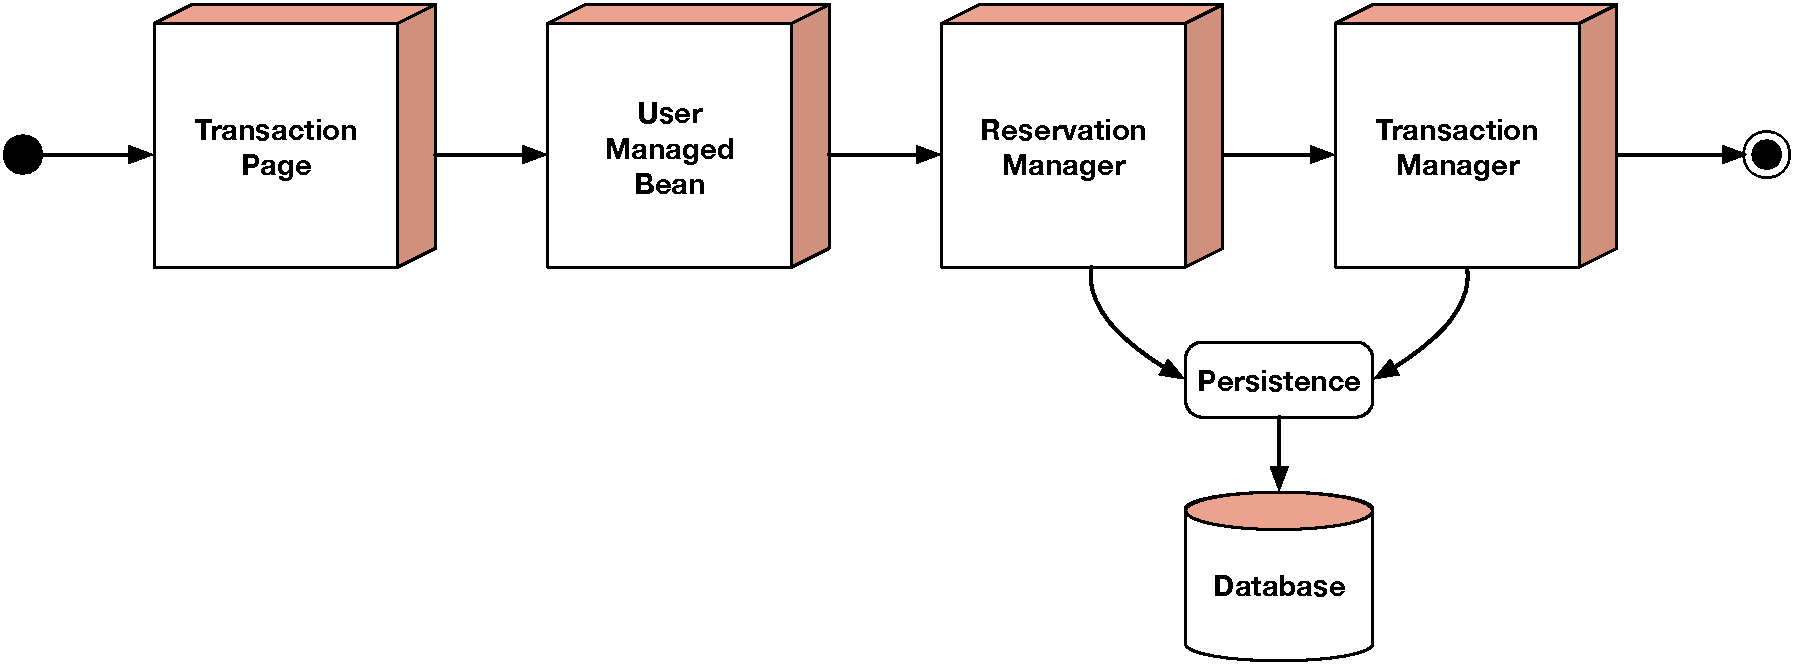
\includegraphics[width=0.85\textwidth]{Images/FeeRun.pdf}
\vspace{10pt}
\caption{Diagram showing the Fee computation and display runtime view}
\label{fig:fee}
\end{figure}
\clearpage

\subsection{Component interfaces} \label{comp-inter}
In this subsection, we are going to identify some of the function offered by the Beans that are present in the Business-tier.

\myparagraph{Visitor Manager} 
\newline
The Figure \ref{fig:visitor} shows the interface of the Visitor Manager, that we think it should expose some methods like:

\begin{itemize}
\item[\textbf{--}] \texttt{createNewUser}: this method adds a new user to the database;
\item[\textbf{--}] \texttt{checkLogin}: this method checks if the nickname and password, provided during the Log In, match and are correct;
\item[\textbf{--}] \texttt{checkRegistration}: this method checks if the personal information, provided during the Registration, are valid.
\end{itemize}

\begin{figure}[htbp]
\centering
\vspace{52pt}
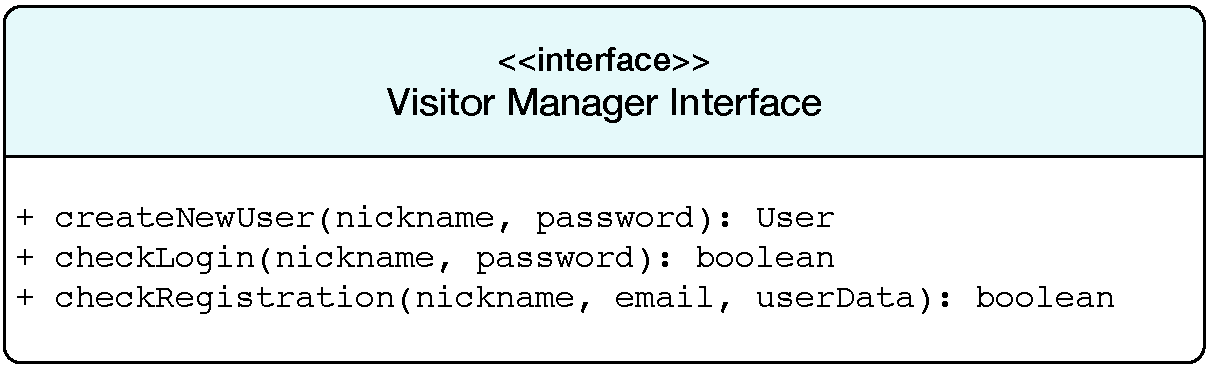
\includegraphics[width=0.85\textwidth]{Images/VisitorManager.pdf}
\vspace{10pt}
\caption{Visitor Manager Interface}
\label{fig:visitor}
\end{figure}
\clearpage

\myparagraph{User Manager} 
\newline
The Figure \ref{fig:user} shows the interface of the User Manager, that we think it should expose some methods like:

\begin{itemize}
\item[\textbf{--}] \texttt{getUserInformation}: this method retrieves all the user information stored in the database;
\item[\textbf{--}] \texttt{setUserInformation}: this method update the user  information stored the database;
\item[\textbf{--}] \texttt{getUserPosition}: this method returns the user position from its smarphone \acs{gps}.
\end{itemize}

\begin{figure}[htbp]
\centering
\vspace{72pt}
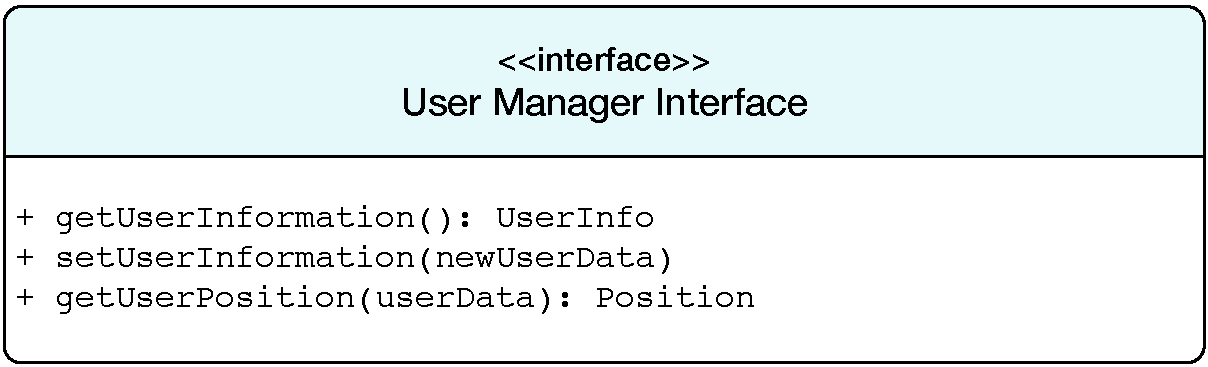
\includegraphics[width=0.85\textwidth]{Images/UserManager.pdf}
\vspace{10pt}
\caption{User Manager Interface}
\label{fig:user}
\end{figure}
\clearpage

\myparagraph{Car Manager} 
\newline
The Figure \ref{fig:car} shows the interface of the Car Manager, that we think it should expose some methods like:

\begin{itemize}
\item[\textbf{--}] \texttt{getCarInformation}: this method retrieves all the car information stored in the database;
\item[\textbf{--}] \texttt{setCarInformation}: this method update the car information stored the database;
\item[\textbf{--}] \texttt{getCarPosition}: this method returns the car position from its \acs{gps} receiver.
\end{itemize}

\begin{figure}[htbp]
\centering
\vspace{72pt}
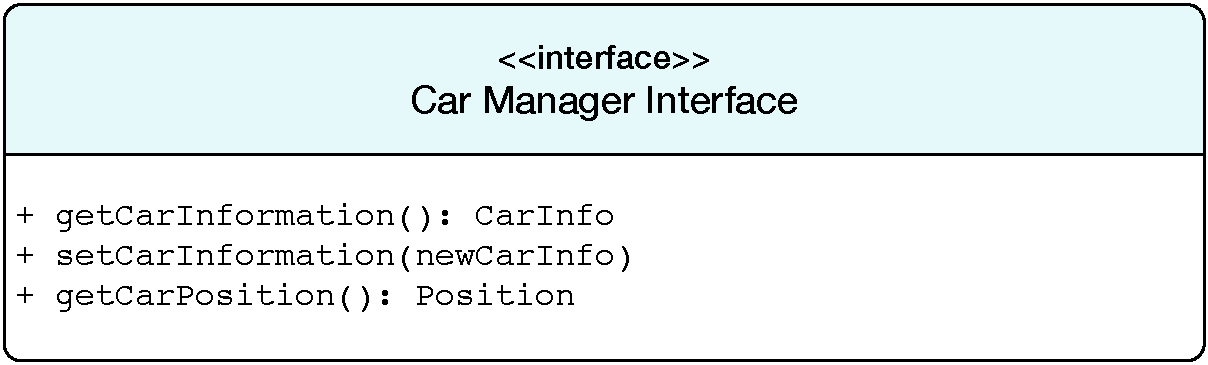
\includegraphics[width=0.85\textwidth]{Images/CarManager.pdf}
\vspace{10pt}
\caption{Car Manager Interface}
\label{fig:car}
\end{figure}
\clearpage

\myparagraph{Reservation Manager} 
\newline
The Figure \ref{fig:reservation} shows the interface of the Reservation Manager, that we think it should expose some methods like:

\begin{itemize}
\item[\textbf{--}] \texttt{createNewReservation}: this method creates a new reservation;
\item[\textbf{--}] \texttt{deleteExistingReservation}: this method deletes an existing reservation;
\item[\textbf{--}] \texttt{getReservationInformation}: this method retrieves all the reservation information stored in the database;
\item[\textbf{--}] \texttt{setReservationInformation}: this method update the reservation information stored the database;
\item[\textbf{--}] \texttt{getReservableCar}: this method retrieves the bookable car near the position given by the user.
\item[\textbf{--}] \texttt{getSafeArea}: this method retrieves the safe area near the position given by the user.
\item[\textbf{--}] \texttt{getPowerGridStation}: this method retrieves the power grid station near the position given by the user.
\end{itemize}

\begin{figure}[htbp]
\centering
\vspace{36pt}
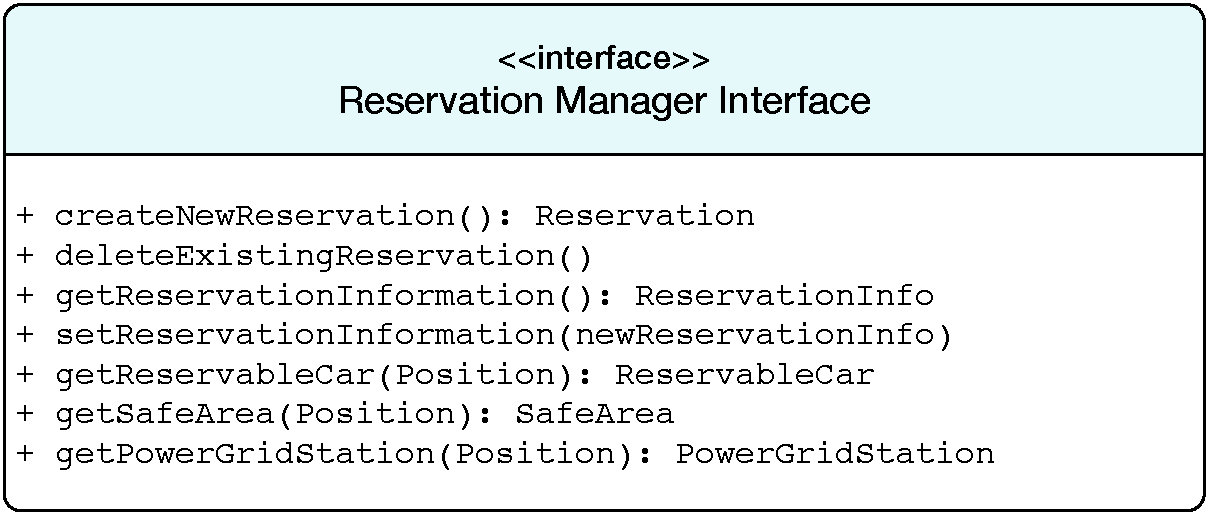
\includegraphics[width=0.85\textwidth]{Images/ReservationManager.pdf}
\vspace{10pt}
\caption{Reservation Manager Interface}
\label{fig:reservation}
\end{figure}
\clearpage

\myparagraph{Transaction Manager} 
\newline
The Figure \ref{fig:transaction} shows the interface of the Transaction Manager, that we think it should expose some methods like:

\begin{itemize}
\item[\textbf{--}] \texttt{getTransactionInformation}: this method retrieves all the transaction information stored in the database;
\item[\textbf{--}] \texttt{setTransactionInformation}: this method update the transaction information stored the database;
\item[\textbf{--}] \texttt{applyDiscountOrPenalties}: this method, after having computed the eventual discount or penalties, applies them.
\end{itemize}

\begin{figure}[htbp]
\centering
\vspace{72pt}
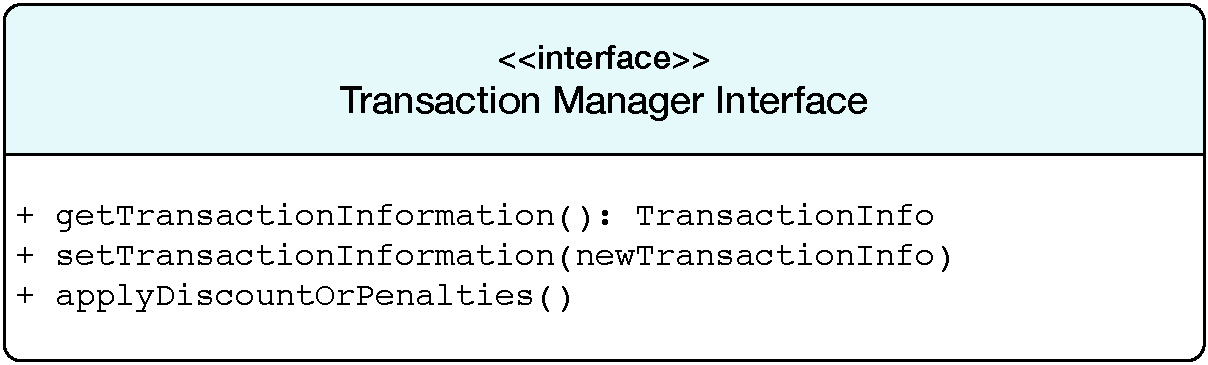
\includegraphics[width=0.85\textwidth]{Images/TransactionManager.pdf}
\vspace{10pt}
\caption{Transaction Manager Interface}
\label{fig:transaction}
\end{figure}
\clearpage

\subsection{Selected architectural styles and patterns} \label{arch-styles}
%Please explain which styles patterns you used, why, and how

In this document, we give the reader a first overview on the architecture of our system and a general and simplified description of its behaviour.
As far as the architecture is concerned, we choose as a model the one of \acl{jee} 7. We think that a 4-tier architecture like this, that also relies on the \acs{mvc} pattern, is the one that best fits our system, since this way we can obtain the performance, scalability, reliability, availability and security requested for PowerEnjoy, a car sharing application.
Moreover, we decide to keep the initial model simple in order to leave the space for further improvements and a more detailed one later in the development.

%\subsection{Other design decisions} \label{other-des}
